\documentclass[fontsize=12pt,paper=a4,twoside=semi,parskip=half-,headsepline,headinclude]{scrreprt}
% Grundgröße 12pt, zweiseitig
\usepackage[headsepline,automark]{scrlayer-scrpage}
% Seitenköpfe automatisch 
\usepackage[ngerman]{babel}
% Sprachpaket für Deutsch (Umlaute, Trennung,deutsche Überschriften)
\usepackage{blindtext}
% macht nur den Blindtext, den Sie aktuell sehen
\usepackage{lmodern}
% schöne PDF-Schrift
\usepackage{graphicx,hyperref,amssymb}
%Graphikeinbindung, Hyperref (alles klickbar, Bookmarks),
%Math. Symbole aus AmsTeX
\usepackage[utf8]{inputenc}
% Umlaute und über Tastatur einzugeben
\usepackage{listings}
% nette Listing-Formatierung
\usepackage[backend=biber]{biblatex}
\addbibresource{literatur.bib}

% Festlegung Kopf- und Fußzeile     
\defpagestyle{meinstil}{%
{\headmark \hfill}
{\hfill \headmark}
{\hfill \headmark\hfill }
(\textwidth,.4pt)
}{%
(\textwidth,.4pt)
{\pagemark\hfill Philipp Ermer}
{\today \hfill \pagemark}
{\today\hfill\pagemark} 
}
\pagestyle{meinstil} 

\raggedbottom
\renewcommand{\topfraction}{1}
\renewcommand{\bottomfraction}{1}

 
%%%%%%%%%%%%%%%%%%%%%%%%%%%%%%%%%%%%%%%%%%%%%%%%%%%%%%%%%%%%%%%%%%%%%%%%%%
\begin{document}    % hier gehts los
  \thispagestyle{empty} % Titelseite

\includegraphics[width=0.2\textwidth]{hsh_icons/Wortmarke_WI_schwarz}

   {  ~ \sffamily
  \vfill
  {\Huge\bfseries Performance-Vergleich von \\Nebenläufigkeits-Konzepten in \\objektorientierten Programmiersprachen}
  \bigskip

  {\Large 
  Philipp Ermer \\[2ex]
 Master-Arbeit im Studiengang "`Angewandte Informatik"' 
 \\[5ex]
   \today } 
}
 \vfill
  
  ~ \hfill
  
\includegraphics[height=0.3\paperheight]{hsh_icons/H_WI_Pantone1665} 

\vspace*{-3cm}


\newpage 
\thispagestyle{empty}
\quad 


  \newpage \thispagestyle{empty}
 \begin{tabular}{ll}
{\bfseries\sffamily Autor} &  Philipp Ermer \\ 
            & Matrikelnummer: 1313395 \\
            & philipp.ermer@web.de \\[5ex]
{\bfseries\sffamily Erstprüfer:} & Prof. Dr. Holger Peine \\
          & Abteilung Informatik, Fakultät IV \\
         & Hochschule Hannover \\
        & holger.peine@hs-hannover.de \\[5ex]
{\bfseries\sffamily Zweitprüfer:} &Prof. Dr. Robert Garmann \\
          & Abteilung Informatik, Fakultät IV \\
         & Hochschule Hannover \\
        & robert.garmann@hs-hannover.de
\end{tabular}

\vfill

%%%%%%%%%%%%%%%%%%%%%%%%%%%%%%%%%%%%%%%%%%%%%%%%%%%%%%%%%%%%%%%%%%%%%%%%%%%%%%%
% Die folgende Lizenz kann die weitere Verwertung Ihrer Arbeit vereinfachen.
% Wenn Sie Ihre Arbeit nicht unter dem genannten Lizenzvertrag lizenzieren
% möchten, können Sie diesen Abschnitt entfernen.
% Dies hat keinerlei Einfluss auf die Bewertung Ihrer Arbeit.
Soweit nicht anders gekennzeichnet, ist dieses Werk unter einem
Creative-Commons-Lizenzvertrag Namensnennung 4.0 lizenziert.
Dies gilt nicht für Zitate und Werke, die aufgrund einer anderen Erlaubnis
genutzt werden.
Um die Bedingungen der Lizenz einzusehen, folgen Sie bitte dem Hyperlink:\\
\url{https://creativecommons.org/licenses/by/4.0/deed.de}

\vfill
%%%%%%%%%%%%%%%%%%%%%%%%%%%%%%%%%%%%%%%%%%%%%%%%%%%%%%%%%%%%%%%%%%%%%%%%%%%%%%%

\begin{center} \sffamily\bfseries Selbständigkeitserklärung \end{center}
% fett und zentriert in der minipage

Hiermit erkläre ich, dass ich die eingereichte Master-Arbeit
selbständig und ohne fremde Hilfe verfasst, andere als die von mir angegebenen Quellen
und Hilfsmittel nicht benutzt und die den benutzten Werken wörtlich oder
inhaltlich entnommenen Stellen als solche kenntlich gemacht habe. 
\vspace*{7ex}

Hannover, den \today \hfill Unterschrift


\newpage 
\thispagestyle{empty}
\quad 
\newpage


  \pdfbookmark[0]{Inhalt}{contents}
  \tableofcontents  % Inhaltsverzeichnis

\listoffigures      % Abbildungsverzeichnis

\listoftables       % Tabellenverzeichnis

\chapter{Einführung}

\section{Motivation}

\section{Ziel der Arbeit}

\section{Verwandte Arbeiten}

\section{Methodik}

\section{Gliederung und Aufbau}



\chapter{Nebenläufigkeitskonzepte}

TODO: Einleitungs-Text Kapitel Nebenläufigkeit

\section{Java: Plattform Threads}

Die bisher verwendeten Java Threads werden auch als Platform Threads bezeichnet, da sie sogenannte Wrapper sind, welche einen Betriebssystem Thread umschließen. Das bedeutet, dass für jeden Platform Thread ein Betriebssystem Thread erstellt wird, welcher dann von einem Java Platform Thread umschlossen wird. Das hat zur Folge, dass Plattform Threads schwergewichtig werden, da Betriebssystem Thread ressourcenintensiv sind und ihre maximale Anzahl damit begrenzt ist. Dies führt dazu, dass die Anzahl der Threads, weit vor anderen Ressourcen, zum limitierenden Faktor wird. Ein weiteres Problem ist, dass die Verwaltung der Threads
vom Betriebssystem übernommen wird und die JRE(Java Runtime Environment) keinen Einfluss darauf nehmen kann. Die Verwaltung der Threads auf Betriebssystemebene muss jedoch sehr allgemein gehalten werden, da sie nicht nur für Java, sondern für alle Programmiersprachen funktionieren muss.

TODO: Pooling? Senkt kosten zum erstellen, erhört nicht die maximale Anzahl an Threads

TODO: Zeichnung Platform Threads

\section{Java: Virtual Threads}

Die Java Virtual Threads sind seit dem JDK 21 (Java Development Kit) fester Bestandteil von Java, sie wurden ursprünglich im Rahmen des Project Loom als sogenannte Fiebers entwickelt. Das Ziel war es die mittlerweile nicht mehr zeitgemäßen Java Threads, durch eine leichtgewichtigere Variante zu ersetzen, welche auf die gleiche API(Application Programming Interface) zurückgreift.

Das Ziel von Virtual Threads besteht in der Umgehung der Schwachstellen von Platform Threads, indem eine große ANzahl Virtual Threads auf eine kleine Zahl Betriebssystem Threads verteilt wird. Dadurch kann eine deutlich größere Anzahl an Virtual Threads gleichzeitig erstellt werden, welche von der JRE verwaltet werden.

Im Detail sieht dies wie folgt aus:

Es wird eine kleine Anzahl an Platform Threads(Wrapper) erstellt, die ihrerseits einen Betriebssystem Thread umschließen. Diese Platform Threads werden als Carrier Threads bezeichnet und ihre Anzahl entspricht standardmäßig der Anzahl der Prozessorkerne des ausführenden Systems. Die Carrier Threads werden von einem ForkJoinPool verwalten der nach dem FIFO(First In - First Out) Prinzip und mit work-stealing arbeitet. 

Für jede neue Aufgabe(task) im System, die nebenläufig ausgeführt werden kann, wird ein neuer Virtual Thread erstellt. Die Aufgabe bleibt dabei die ganze Zeit im gleichen Virtual Thread. Der Virtual Thread wiederum wird zum bearbeiten der Aufgabe in einen Carrier Thread eingesetzt(mount). 

TODO: Zeichnung Virtual Threads

Dort bleibt der Virtual Thread so lange bis die Aufgabe abgeschlossen ist oder der Thread blockiert. Sollte es zu einer Blockade, zum Beispiel durch eine I/O-Operation, kommen, wird der Virtual Thread aus dem Carrier Thread entnommen(unmount) und so lange geparkt bis er nicht mehr blockiert ist und die Bearbeitung der Aufgabe fortgesetzt werden kann. Der Virtual Thread wir dann wieder in eine freien Carrier Thread eingesetzt werden, dies kann aber ein andere sein als zu Beginn. Daraus folgt, eine Aufgabe wird ihre gesamte Lebenszeit vom gleichen Virtual Thread ausgeführt, welcher jedoch in unterschiedlichen Carrier Threads eingesetzt werden kann. Die hat den Vorteil, dass ein Virtual Thread ein Betriebsystems Thread nur dann benutzt, wenn der Virtual Thread Berechnungen auf dem Prozessor ausführt. Ist ein Virtual Thread blockiert macht er platzt auf dem Betriebsystem Thread für einen anderen Virtual Thread. Dies führt zu einer effizienteren auslastung des Prozessors.

TODO: Zeichnung Virtual Threads Ablaufdiagramm

Ein typischer Anwendungsfall für Virtual Threads ist ein Server-Anwendung die Anfragen im Thread per request Model bearbeitet. Für jede neue Anfrage wird ein neuer Thread erstellt der diese Anfrage bearbeitet. So können mehrere Anfragen nebenläufig berarbeitet werden. Dies bedeutet bei Platform Threads, dass für jede neue Anfrage nicht nur ein neuer Platform Thread sondern auch ein neuer Betriebssystem Thread erstellt werden muss. Da die Anzahl an Betriebssystem Thread aber für ein System stark limitiert ist, in der Regel einige Tausend, ist damit auch die Anzahl der nebenläufig zu bearbeitenden Anfragen limitiert. So werden Plarform Threads zum limitierenden Faktor des Systems. Virtual Threads hingegen sind deutlich leichtgewichtiger, da ihre Anzahl nicht an die zur Verfühgung stehenden Betriebssystem Threads gebunden ist. Dadurch lässt sich eine Große Anzahl von ihnen erstellen, bis zu mehrere Millionen.

Der Vorteil von Virtual Thread gegenüber Platform Threads bei dem Thread per request Model, lässt sich gut mit Littels Gesetz zeigen. Es besagt, dass die sich gleichzeitig in Bearbeitung befindlichen Aufgaben davon abhängig ist wie hoch der Durchsatz($\lambda$) und die Durchlautzeit (W) sind.

TODO: Formel

Daraus folgt, das der Durchsatz sich aus den gleichzeitig in Bearbeitung befindlichen Aufgaben und der Durchlaufzeit errechnet.

TODO: umgestelle Formel

Auf das Thread per request Model angewandt, bedeutet das der Durchsatz die pro Sekunde in das System eingehend Anfragen ist. Die Durchlaufzeit wird dadurch beschrieben wie hoch die durchschnittlich Latenz des Systems ist um eine Anfrage zu beantworten. 

Gehen wir also von einem System aus, das 200 Anfragen pro Sekunde verarbeitet, bei einer Latenz von 50ms pro Anfrage. Dafür ist es nötig 10 Anfragen gleichzeitig nebenläufig zu verarbeiten. Soll das System nun auf 2000 Anfragen pro Sekunde, bei gleichbleibender Latenz skaliert werden, muss das System nun 100  Aufgeben gleichzeitig nebenläufig verarbeiten.

Da wir vom Thread per request Model ausgehen, müssen also im Fall von  Platform Threads, 100 von ihnen erstellt werden und damit auch 100 Betriebssystem Threads. Somit ist die Skalierbarkeit auf die maximal zur Verfühgung stehenden Betriebssystem Threads(einige Tausend) begrenzt. Virtual Threads hingegen lassen sich in einer deutlich größeren Anzahl erstellen(mehrere Millionen) und werden so nicht zum limitierenden Faktor wenn es um die Skalierbarkeit des beschriebenen Beispiels geht.

Die Annahme stimmt allerdings nur so, wie die nebenläufig bearbeiteten Aufgaben, weiterhin mit der gleichen Latenz bearbeitet werden. Dies ist der Fall, wenn ein Aufgabe pausiert um beispielsweise auf I/O-Operation zu warten. Wenn die einzelne Aufgaben jedoch rechenintensiv sind und möglicherweise niemals pausieren verlieren Virtual Threads ihren Vorteil gegen über Platform Threads. Virtual Threads können nicht einzelne Aufgaben schneller ausführen als Platform Threads, sondern mehr Aufgaben nebenläufig Aufgaben. Damit lässt sich abschließend sagen Virtual Threads steigern den Durchsatz einer Anwendung gen über Platform Threads, wenn viel Aufgaben nebenläufig ausgeführt werden und die rechenlast der einzelnen Aufgaben niedrig ist.


VT mount/ unmount
JDK rewritten where blocking
continuations .yield()
blocking I/O operation automatically suspends the virtual thread until it can be resumed later

pinning (schlecht)
VT kann nicht unmounted werden
native call
synchronized code block
-kurze Zeit kein Problem
-sonst reentrant lock
-zukünftig vermutlich gelöst

platform threads, implemented as wrappers for OS threads (1:1 scheduling). Virtual threads employ M:N scheduling, where a large number (M) of virtual threads is scheduled to run on a smaller number (N) of OS threads.

VT seit JDK 19 previe(alte JEP)
Einsatz auf mehrkernprozessoren

Einfache Programmierung
Gleiche Trhread API
java.lang.Thread API
Können integriert werden ohne bestehende Codebasis wesentlich zu verändern
TODO:Code Beispiel
Virtual threads are cheap and plentiful, and thus should never be pooled: 
A new virtual thread should be created for every application task
virtual threads will thus be short-lived and have shallow call stacks
Platform threads, by contrast, are heavyweight and expensive


PT erstellen kostet Zeit Speicher
2 MB pro PT (20 MB?)
~ 1 Ms
~100 ns context switch(OS abhängig)

PT
einige hundert
VT
Millionen(fast unbegrenzt)

VT= Daemon threads

Virtual Threads \cite{Karsten2020}

\section{Java: Completable Futures}

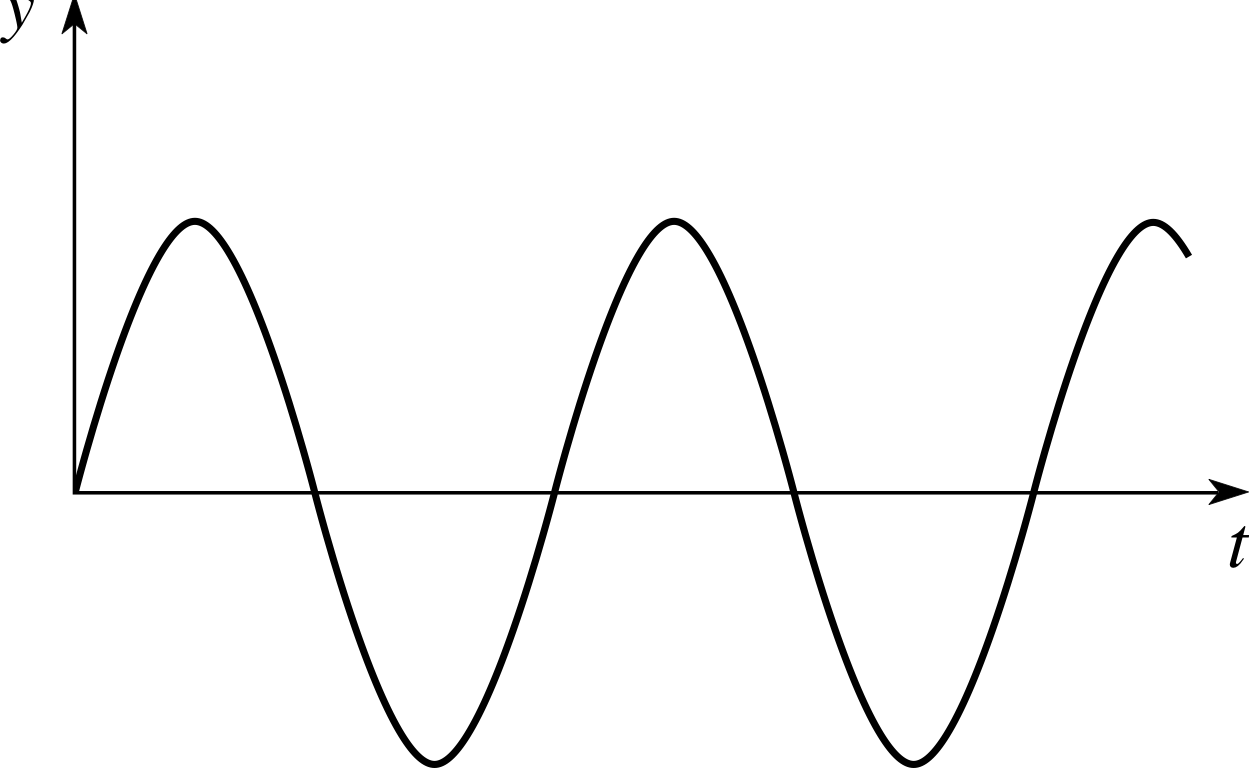
\includegraphics[scale=2.5]{figures/example.png}

\section{Kotlin: CO-Routinen}

\section{Kotlin: Threads}

\section{Go: Go-Routinen}

\section{C\#: async/await}

\section{Vergleich der Konzepte}



\chapter{Benchmarks}

\section{Benchmark 1}

\section{Benchmark 2}

\section{Benchmark 3}

\section{Benchmark 4}



\chapter{Testaufbau}

\section{Testumgebung}

\section{Performancefaktoren}

\section{Werkzeuge zur Datenerhebung}



\chapter{Messungen}

\section{Messung: Benchmark 1}

\section{Messung: Benchmark 2}

\section{Messung: Benchmark 3}

\section{Messung: Benchmark 4}



\chapter{Auswertung}

\section{Ergebnisse und Beobachtungen}

\section{Diskussion und Bewertung}



\chapter{Zusammenfassung und Ausblick}

\section{Zusammenfassung}

\section{Ausblick}



\printbibliography


%\input{abkuerz.tex}      % Einbinden von Tex-Files
%\input{einfuehrung.tex}
%
%\include{normen}        % Einbinden von größeren Tex-Files,z.B. Kapiteln
%\include{aufbau}
%\include{zitieren}
%\include{form}
%\include{allgtips}
%
%\bibliographystyle{alpha}  % Schlüssel als Buchstaben
%\bibliography{literaturverzeichnis}      % Literaturverzeichnis

\end{document}


